\chapter{實驗結果與分析}
{
本章節將介紹第三章提到的資料集於本實驗中 training data 與 test data 之分配方式,以及介紹評估實驗結果之方法。最後比較基於監督式學習與透過對使用者分群之後再以監督式學習之預測結果,並對實驗結果提出結論與分析。
}

\section{實驗資料集介紹}
{
基於第三章所介紹的資料集,本實驗透過交叉驗證(5-fold cross validation)的方式,將資料集依據使用者分割成 5 份子樣本,將其中 1 份單獨的子樣本當作驗證模型的資料,而其他 4 份子樣本用來訓練模型,重複 5 次,將每一份子樣本都進行驗證 1 次,最後將 5 次驗證結果取平均,最後得到 1 個能夠評估此模型的單一值。


}

\section{評估模型優劣之方法}
{
由於使用者個人資訊之預測屬於多類別(multi-class)之分類問題,而使用者大六性格特質分數之預測屬於數值回歸問題,兩者所使用的評估標準不相同,因此本節將針對兩種不同問題的預測模型分別進行評估方法之介紹。


}
\subsection{個人資訊預測結果之評估標準}
{
基於分類問題,大部分以 $F_1$ score 進行準確度評估,$F_1$ score 主要在召回率(recall)與精確率(precision)之間取得平衡,透過圖~\ref{fig:dtt} 中定義的 TP、FP、FN、TN 來進行召回率、精確率以及 $F_1$ score 之計算,其公式如下。\par

$$F_1 \mbox{ } score = 2 \cdot \frac{precision \cdot recall}{precision + recall} \eqno{(5.1)}$$

$$Precision = \frac{tp}{tp+fp} \eqno{(5.2)}$$

$$Recall = \frac{tp}{tp+fn} \eqno{(5.3)}$$

\begin{figure}[h]
    \graphicspath{{fig/}}
    \begin{center}
    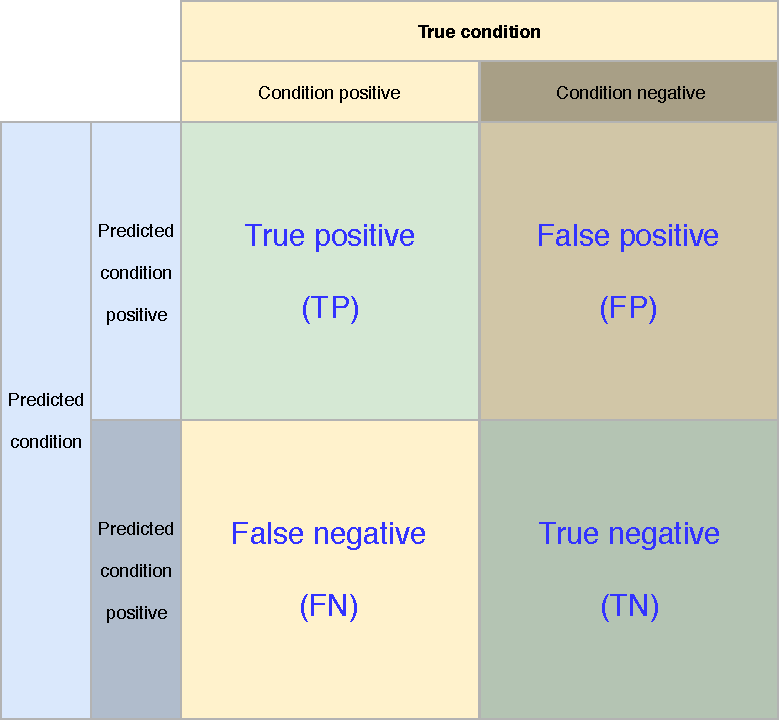
\includegraphics[scale=0.7]{fig/dtt.pdf}
    \caption{diagnostic testing table}
    \label{fig:dtt}
    \end{center}
\end{figure}


而本實驗中預測使用者之個人資訊為 multi-class 分類方法,因此無法直接使用 $F_1$ score 當作評估標準,必須改以 $MicroF_1$ 與 $MacroF_1$ 對 multi-class 分類進行評估,其公式如式 5.4、5.5, $MicroF_1$ 將 TP、FP、FN、TN 各進行累加後再計算其 $F_1$ score,而 $MacroF_1$ 則是將每一種類別之 $F_1$ score 計算出來後再取平均。其中 $MicroF_1$ 與 $MacroF_1$ 最明顯的差異在於,$MicroF_1$ 較不考慮每一種類別之間的樣本數量的平衡狀況,而在 $MacroF_1$ 的計算方式下,樣本數較少的類別對於整體分數的影響等同於其他類別,因此再選擇評估標準時,必須考慮資料集中樣本類別間是否平均,而本實驗所使用之資料集,每一種類別之樣本數較為不平衡,因此選擇以 $MicroF_1$ 作為評估標準。

$$MicroF_1=\frac{2\cdot \sum_{i=1}^C{TP_i}}{2\cdot \sum_{i=1}^C{TP_i} + \sum_{i=1}^C{FP_i} + \sum_{i=1}^C{FN_i}} \eqno {(5.4)}$$

$$MacroF_1 = \frac{1}{C} \sum_{i=1}^C{\frac{2\cdot TP_i}{2\cdot TP_i+FP_i+FN_i}} \eqno {(5.5)}$$




}

\subsection{大六性格特質分數預測結果之評估標準}
{
對於數值預測結果之評估標準,本篇論文以均方根誤差(root-mean-square error)進行評估,$RMSE$ 為一種經常用來測量數值之間差異性的量度,其計算方式如式 5.6,其中 $\hat{y}$ ̂為樣本實際值、$y$ 為預測值、$n$ 為預測樣本總數。

$$RMSE = \sqrt{\frac{ \sum_{t=1}^n{(y_t-\hat{y_t})^2 }}{n}} \eqno{(5.6)}$$

}

\subsection{使用者分群效果之評估標準}
{
第四章中介紹藉由 k-means 將使用者進行分群,本篇論文選擇 Silhouette score~\cite{de2015recovering}作為分群效果之評估標準。式 5.7 中 $s(i)$ 為第 i 位使用者之 Silhouette score,$a(i)$ 為第 i 位使用者與同群之其他使用者之間的平均距離,$b(i)$ 為使用者 $i$ 與不同群之其他使用者間的最小平均距離。而式 5.7 等價於式 5.8 因此可以了解當 $s(i)=0$ 時表示第 $i$ 位使用者剛好介於兩群之交界處,若 $s(i)<0$ 則表示第 $i$ 位使用者介於兩群之重疊處,因此當 Silhouette score $<0$ 則表示分群效果不佳。

$$s(i)= \frac{b(i)-a(i)}{\max (a(i),b(i))} \eqno{(5.7)}$$

\begin{equation}
\setcounter{equation}{8}
s(i)=
\left\{
     \begin{array}{lr}
     1-\frac{a(i)}{b(i)}, & \mbox{if }a(i)<b(i)\\  
     0, & \mbox{if }a(i)=b(i)\\  
     \frac{b(i)}{a(i)}-1, & \mbox{if }a(i)>b(i)    
     \end{array}
\right .
\end{equation}
}

\section{預測個人資訊之結果比較}
{
本節將介紹 4 種分類器:k-NN、Random forests、Logistic regression 以及 SVM 之參數設定,並在最後透過混淆矩陣(confusion matrix)以及 $MicroF_1$ 之分數比較 “基於監督式學習” 與 “結合分群之監督式學習” 兩者年齡、性別、感情狀態之預測結果。 \par

\clearpage

基於監督式學習之預測方法中,當使用 k-NN 作為分類器時,先利用 $MicroF_1$ 找出最佳k之值,並以此值產生混淆矩陣評估整體預測結果。如圖~\ref{fig:super_knn_microf1},呈現 k-NN 中當 $k$ 之值從 1 增加至 20 其預測年齡、性別、感情狀態之 $MicroF_1$ 分數,其最大值分別為 $k=18$、$k=19$、$k=5$,$MicroF_1$ 分別為 $0.427$、$0.594$、$0.478$,再將 3 種不同的 $k$ 值之 k-NN 預測結果以混淆矩陣呈現,如圖 ~\ref{fig:knn_con} 左側中 y 軸為 true label 值、x 軸為 predicted label,矩陣中間之值為預測樣本數與其比例,透過混淆矩陣可以清楚觀察到各種類之預測狀況。\par

\begin{figure}[h]
    \graphicspath{{fig/}}
    \begin{center}
    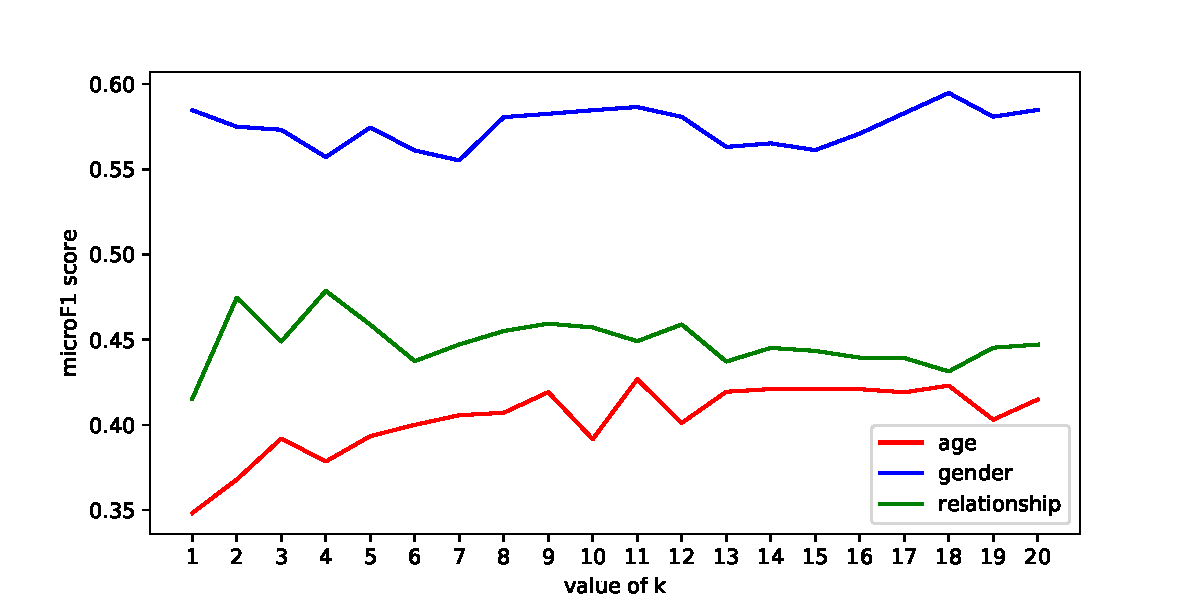
\includegraphics[scale=0.5]{fig/super_knn_microf1.pdf}
    \caption{k-NN 中根據不同 k 值對應之 $MicroF_1$ 分數}
    \label{fig:super_knn_microf1}
    \end{center}
\end{figure}


使用 Random forests 作為分類器時,由於其中決策樹之深度可以進行調整,因此同樣使用 $MicroF_1$ 進行不同最大深度($max \_depth$)之預測效果比較(圖~\ref{fig:super_rf_microf1}),其最佳年齡、性別以及感情狀態之最大深度值分別為 8、5、9,其 $MicroF_1$ 分別為 $0.453$、$0.697$、$0.488$,而最佳深度之混淆矩陣如圖~\ref{fig:rf_con} 左側。\par

\begin{figure}[h]
    \graphicspath{{fig/}}
    \begin{center}
    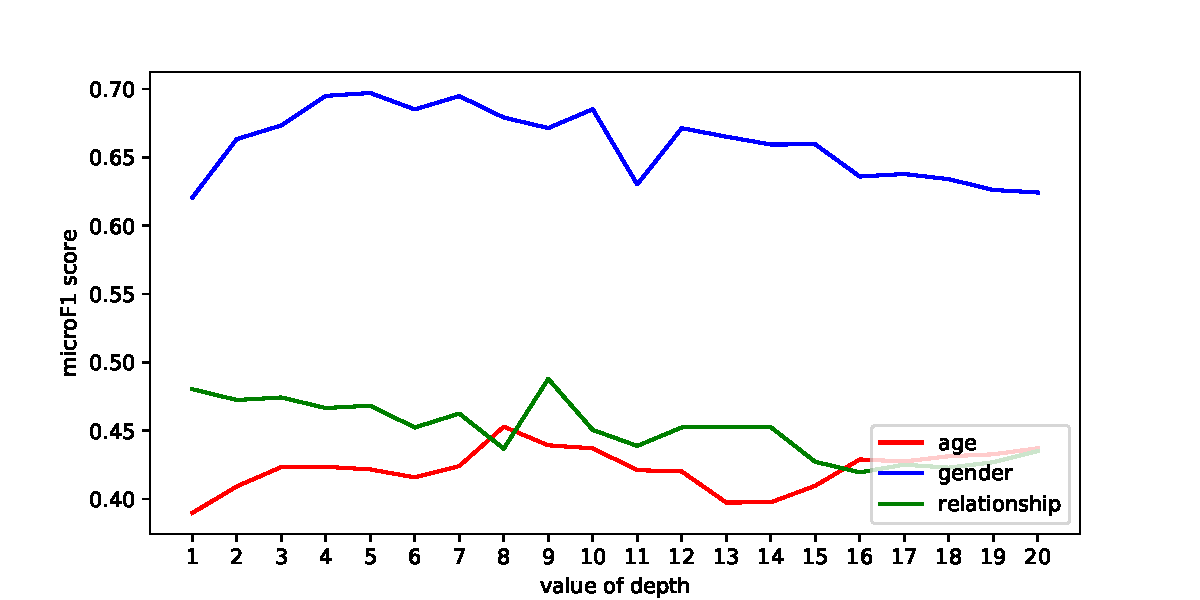
\includegraphics[scale=0.5]{fig/super_rf_microf1.pdf}
    \caption{ Random forests 中根據不同 $max \_depth$ 值對應之 $MicroF_1$ 分數}
    \label{fig:super_rf_microf1}
    \end{center}
\end{figure}
\clearpage

使用 Logistic regression 與 SVM 當作分類器時,能夠透過調整其中 regularization term 之權重($C$)找出最佳預測效果,因此同樣也利用 $MicroF_1$ 找出最佳權重分配, Logistic regression 對年齡、性別、感情狀態預測結果之 $MicroF_1$ 分別為 $0.427$、$0.697$、$0.476$,而 SVM 之預測結果 $MicroF_1$ 分別為 $0.388$、$0.591$、$0.474$,並以混淆矩陣呈現 Logistic regression 預測結果
(圖~\ref{fig:lr_con} 左側)與 SVM 預測結果(圖~\ref{fig:svm_con} 左側)。\par

結合分群之監督式學習的預測方法中,將透過 k-means 將使用者分群並以 Silhouette score 決定分群數量(圖~\ref{fig:silhouette_score} 為 Silhouette score 之分布),由於當 $k<6$ 時 Silhouette score 下降幅度較為明顯,因此本實驗決定將分群數量定為 2 到 6 群,再以 k-NN、Random forests、Logistic regression 以及 SVM 對分群後的使用者進行個人資訊之預測,最後將以 $MicroF_1$ 決定其中分類器之參數設定,並以混淆矩陣呈現預測結果。\par

\begin{figure}[h]
    \graphicspath{{fig/}}
    \begin{center}
    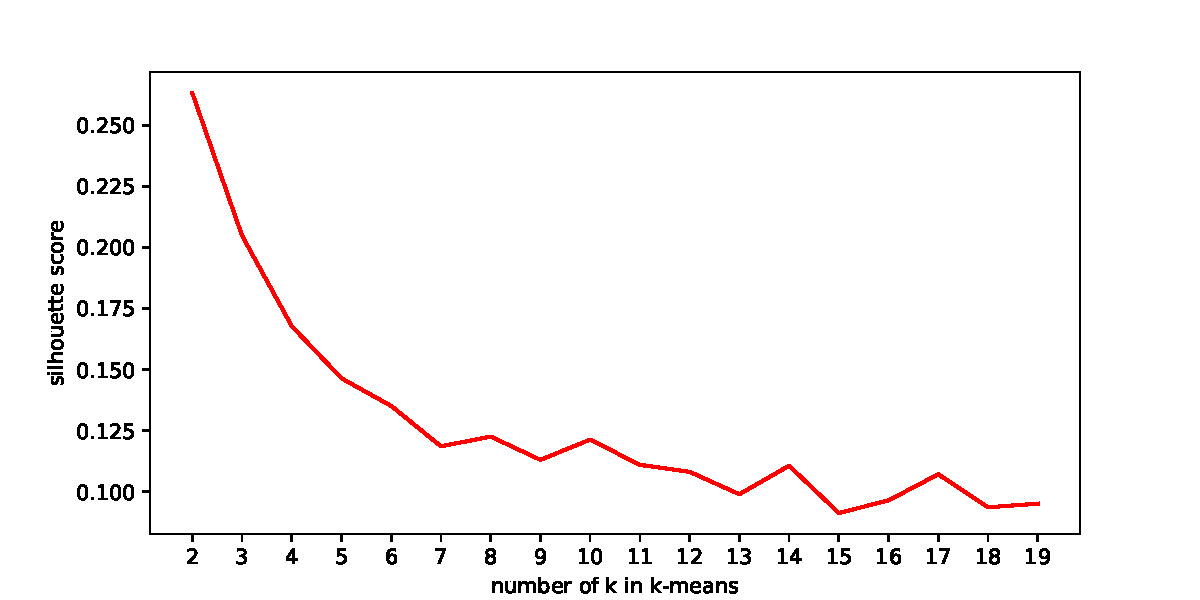
\includegraphics[scale=0.6]{fig/silhouette_score.pdf}
    \caption{分群數量之 Silhouette score 分布}
    \label{fig:silhouette_score}
    \end{center}
\end{figure}

以 k-NN 作為分類器時,年齡之最佳分群數量為 3 群、最佳 $k$ 值為 20,性別之最佳分群數量為 5 群、最佳 $k$ 值為 15,感情狀態之最佳分群數量為 3 群、最佳 $k$ 值為 3,其分群效果以混淆矩陣來表示,如圖 ~\ref{fig:knn_con} 右側。\par

以 Random forests 作為分類器時,年齡之最佳分群數量為 3 群、最佳 $max\_depth$ 值為 20,性別之最佳分群數量為 5 群、最佳 $max\_depth$ 值為 15,感情狀態之最佳分群數量為 3 群、最佳 $max\_depth$ 值為 3,其分群效果以混淆矩陣來表示,如圖~\ref{fig:rf_con} 右側。\par

以 Logistic regression 作為分類器時,年齡之最佳分群數量為 3 群、最佳 $C$ 值為 20,性別之最佳分群數量為 5 群、最佳 $C$ 值為 15,感情狀態之最佳分群數量為 3 群、最佳 $C$ 值為 3,其分群效果以混淆矩陣來表示,如圖~\ref{fig:lr_con} 右側。\par

以 SVM 作為分類器時,年齡之最佳分群數量為 5 群、最佳 $C$ 值為 20,性別之最佳分群數量為 5 群、最佳 $C$ 值為 15,感情狀態之最佳分群數量為 3 群、最佳 $C$ 值為 3,其分群效果以混淆矩陣來表示,如圖~\ref{fig:svm_con} 右側。\par

表~\ref{tab:demo_f1}呈現以 4 種分類器與總是預測使用者數量最多的類別(baseline)中利用 “基於監督式學習” 、 “結合分群監督式學習” 預測年齡、性別、感情狀態之 $MicroF_1$ 分數,透過此表格能夠清楚了解經過分群後預測個人資訊之效能大部分都有提高,對於性別之預測 “基於監督式學習” 有較好的表現,而在年齡、感情狀態之預測 “結合分群監督式學習” 預測較為準確。


\renewcommand{\arraystretch}{1.5}  
\begin{table}[h]  
  
  \centering  
  \fontsize{12}{20}\selectfont  
  \caption{基於監督式學習與結合分群監督式學習之預測 $MicroF_1$ 分數比較表}  
  \label{tab:demo_f1}  
    \begin{tabular}{|c|c|c|c|c|c|c|}  
    \hline  
    \multirow{Classifier}&  
    \multicolumn{3}{c|}{基於監督式學習}&\multicolumn{3}{c|}{結合分群監督式學習}\cr\cline{2-7}  
    &Age&Gender&Relationship&Age&Gender&Relationship\cr  
    \hline  
    \hline  
    Baseline&0.388&0.545&0.474&0.411&0.598&0.476\cr\hline  
   k-NN&0.427&0.594&0.478&0.435&0.618&0.482\cr\hline  
    Random forests&0.453&{\bf 0.697}&0.488&0.419&0.687&{\bf 0.512}\cr\hline  
    Logistic regression&0.427&{\bf 0.697}&0.476&{\bf 0.457}&0.675&0.498\cr\hline  
    SVM&0.388&0.591&0.474&0.411&0.642&{\bf 0.512}\cr\hline
    \end{tabular}  
\end{table}  


\begin{figure*}[h]
    \centering
    \begin{subfigure}
      \centering
      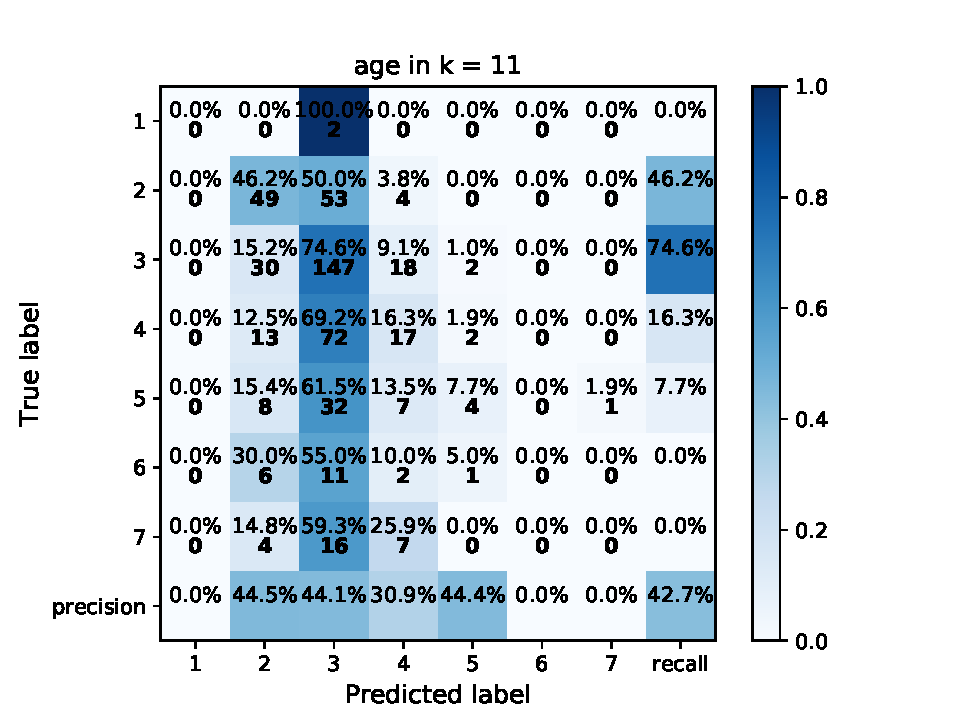
\includegraphics[scale=0.45]{fig/super_knn_age.pdf}
    \end{subfigure}%
    \begin{subfigure}
      \centering
      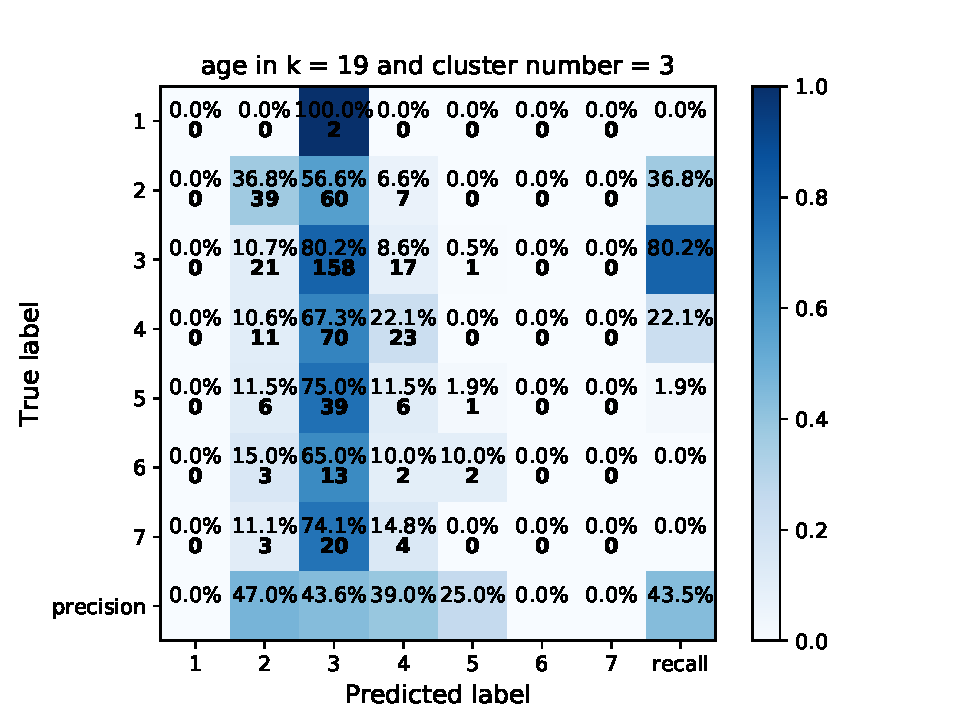
\includegraphics[scale=0.45]{fig/kms_knn_age.pdf}
    \end{subfigure}
\end{figure*}

\begin{figure*}[h]
    \centering
    \begin{subfigure}
      \centering
      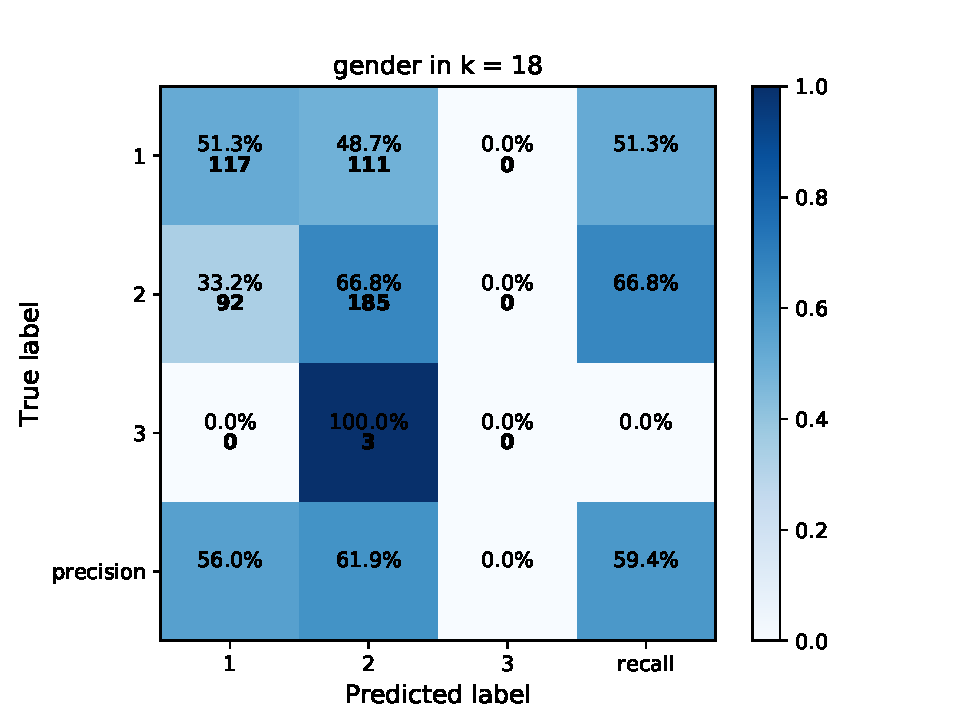
\includegraphics[scale=0.45]{fig/super_knn_gender.pdf}
    \end{subfigure}%
    \begin{subfigure}
      \centering
      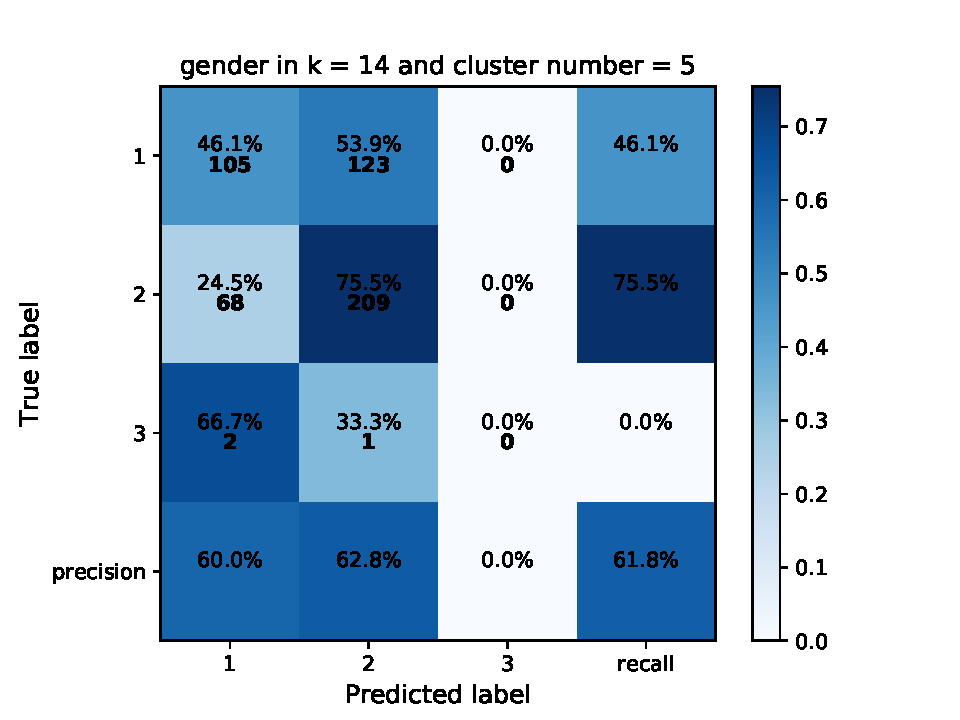
\includegraphics[scale=0.45]{fig/kms_knn_gender.pdf}
    \end{subfigure}
\end{figure*}

\begin{figure}[h]
    \centering
    \begin{subfigure}
      \centering
      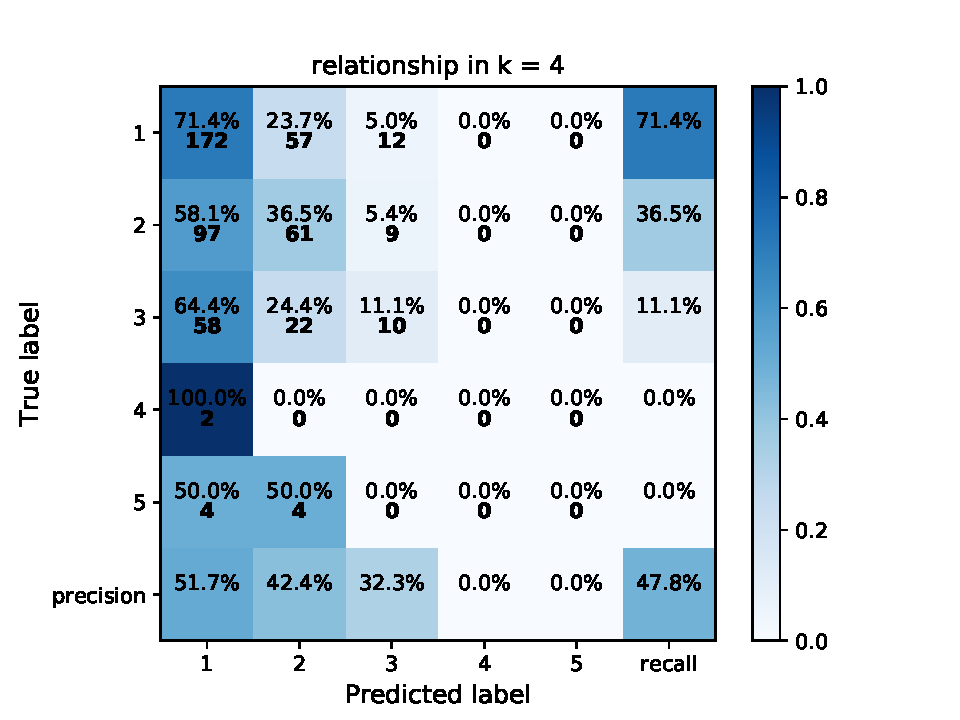
\includegraphics[scale=0.45]{fig/super_knn_relationship.pdf}
    \end{subfigure}%
    \begin{subfigure}
      \centering
      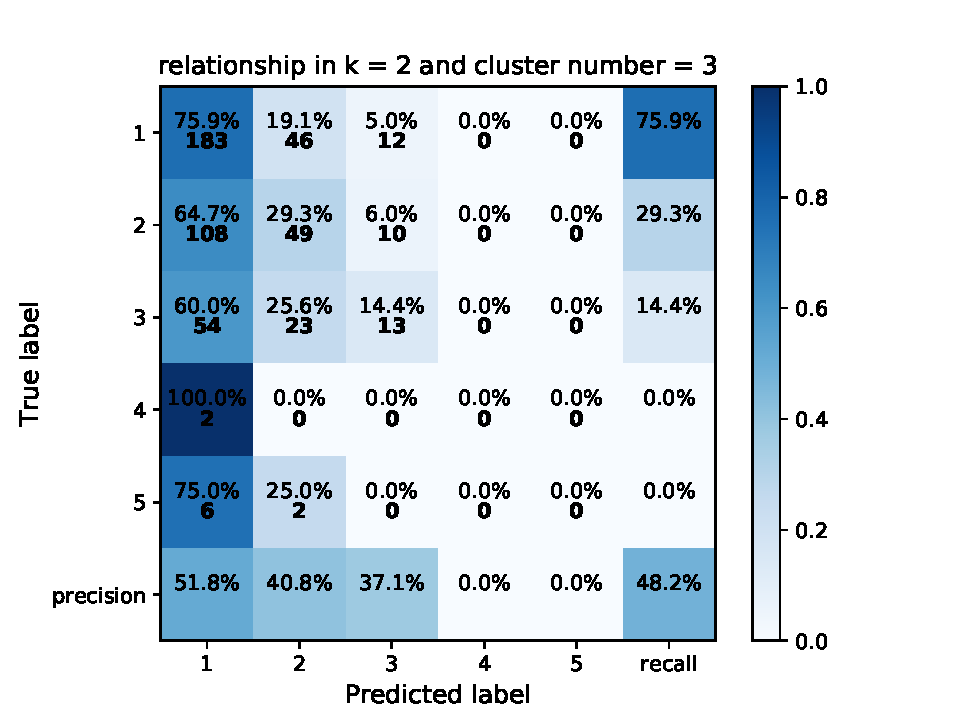
\includegraphics[scale=0.45]{fig/kms_knn_relationship.pdf}
    \end{subfigure}
    \caption{左側為 k-NN 預測個人資訊之混淆矩陣、右側為分群後以 k-NN 預測個人資訊之混淆矩陣}
    \label{fig:knn_con}
\end{figure}

\begin{figure*}[h]
    \centering
    \begin{subfigure}
      \centering
      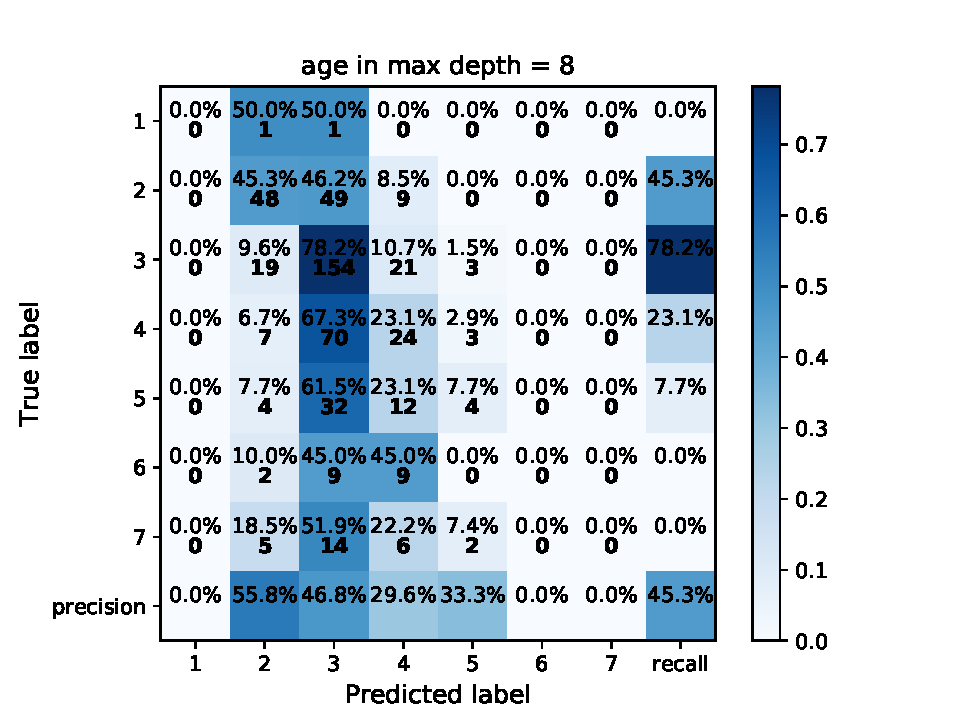
\includegraphics[scale=0.45]{fig/super_rf_age.pdf}
    \end{subfigure}%
    \begin{subfigure}
      \centering
      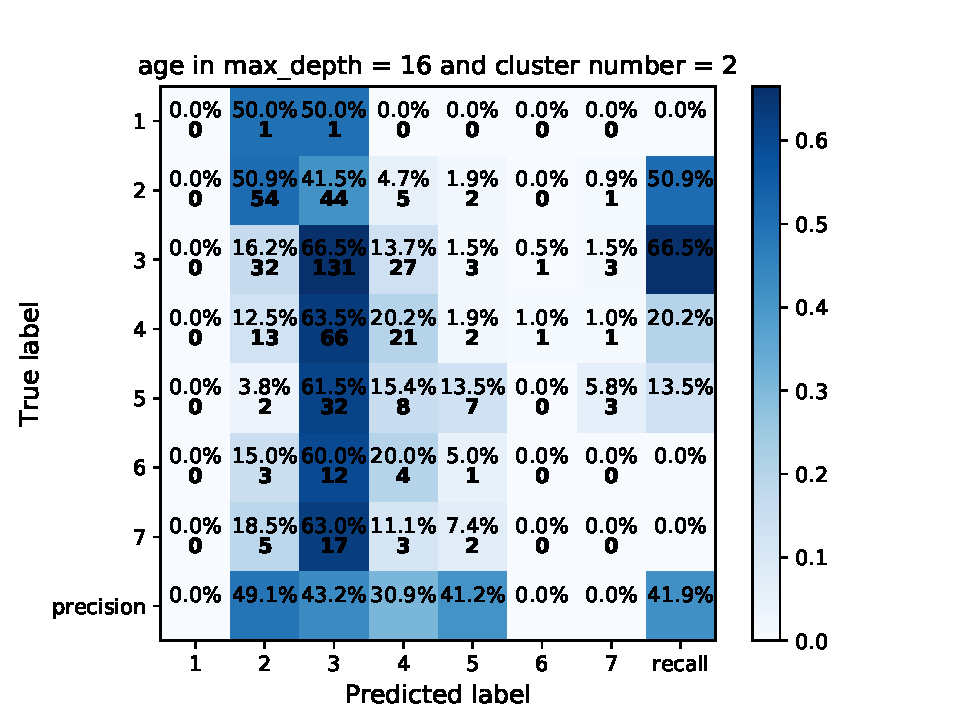
\includegraphics[scale=0.45]{fig/kms_rf_age.pdf}
    \end{subfigure}
\end{figure*}

\begin{figure*}[h]
    \centering
    \begin{subfigure}
      \centering
      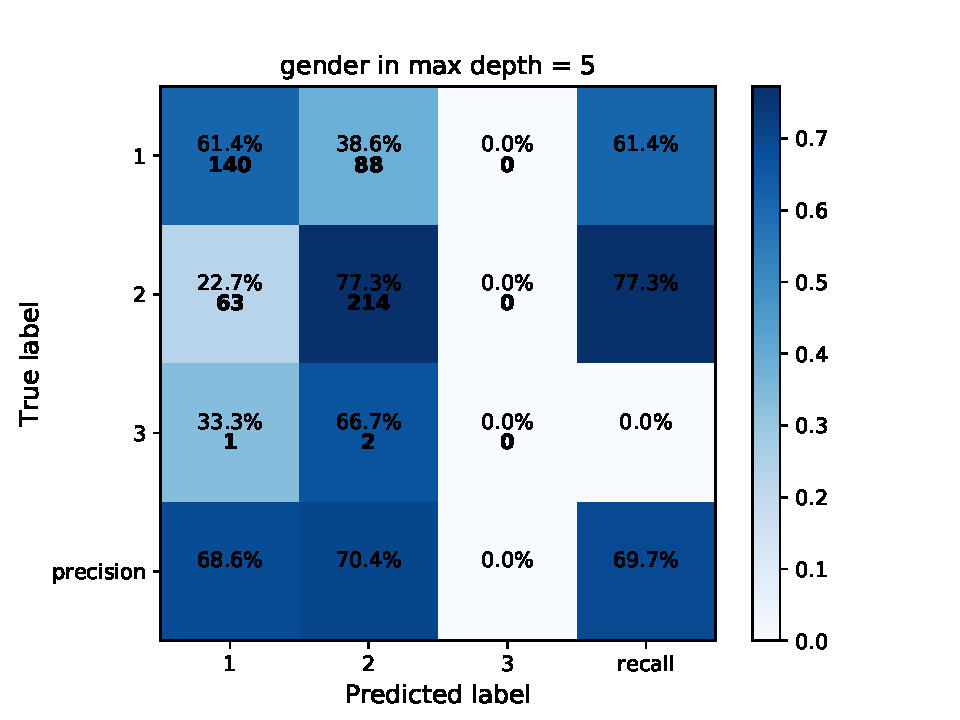
\includegraphics[scale=0.45]{fig/super_rf_gender.pdf}
    \end{subfigure}%
    \begin{subfigure}
      \centering
      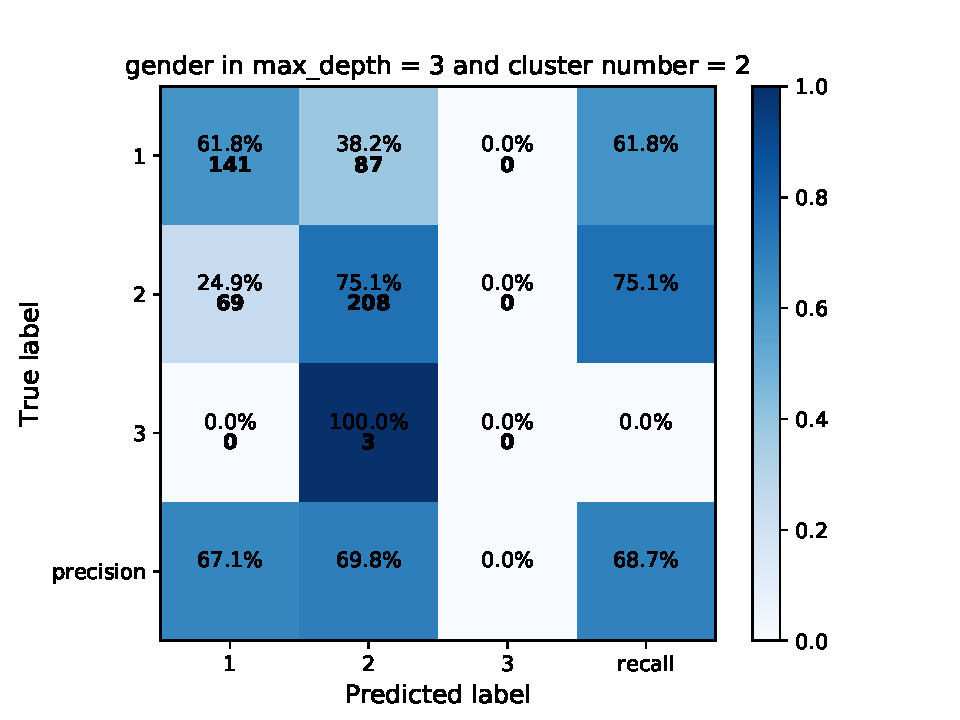
\includegraphics[scale=0.45]{fig/kms_rf_gender.pdf}
    \end{subfigure}
\end{figure*}

\begin{figure}[h]
    \centering
    \begin{subfigure}
      \centering
      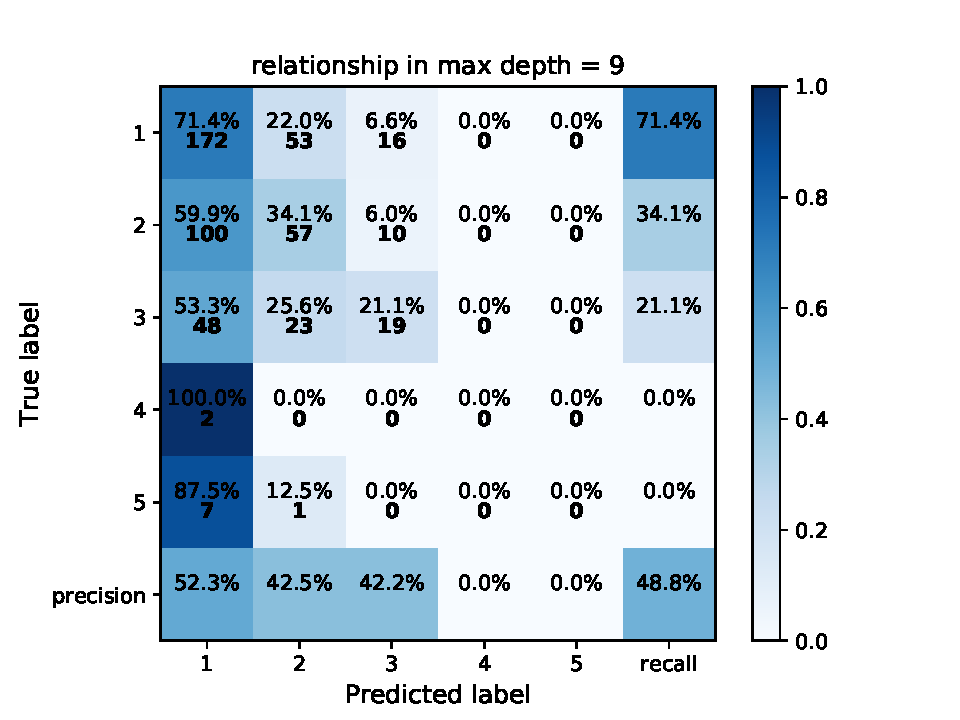
\includegraphics[scale=0.45]{fig/super_rf_relationship.pdf}
    \end{subfigure}%
    \begin{subfigure}
      \centering
      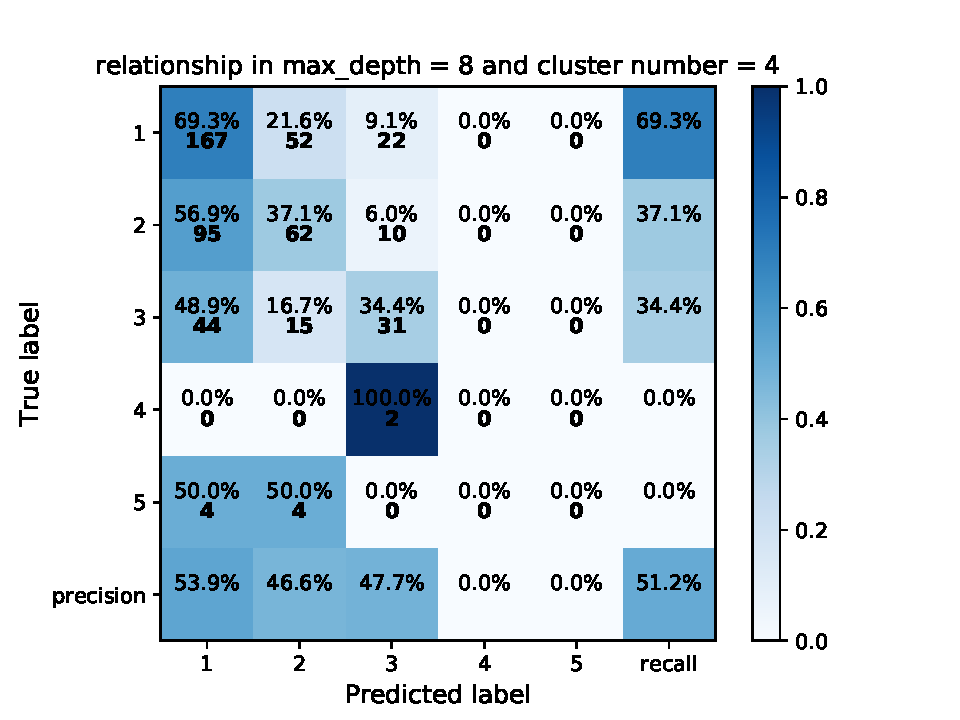
\includegraphics[scale=0.45]{fig/kms_rf_relationship.pdf}
    \end{subfigure}
    \caption{左側為 Random forests 預測個人資訊之混淆矩陣、右側為分群後以 Random forests 預測個人資訊之混淆矩陣}
    \label{fig:rf_con}
\end{figure}

\begin{figure*}[h]
    \centering
    \begin{subfigure}
      \centering
      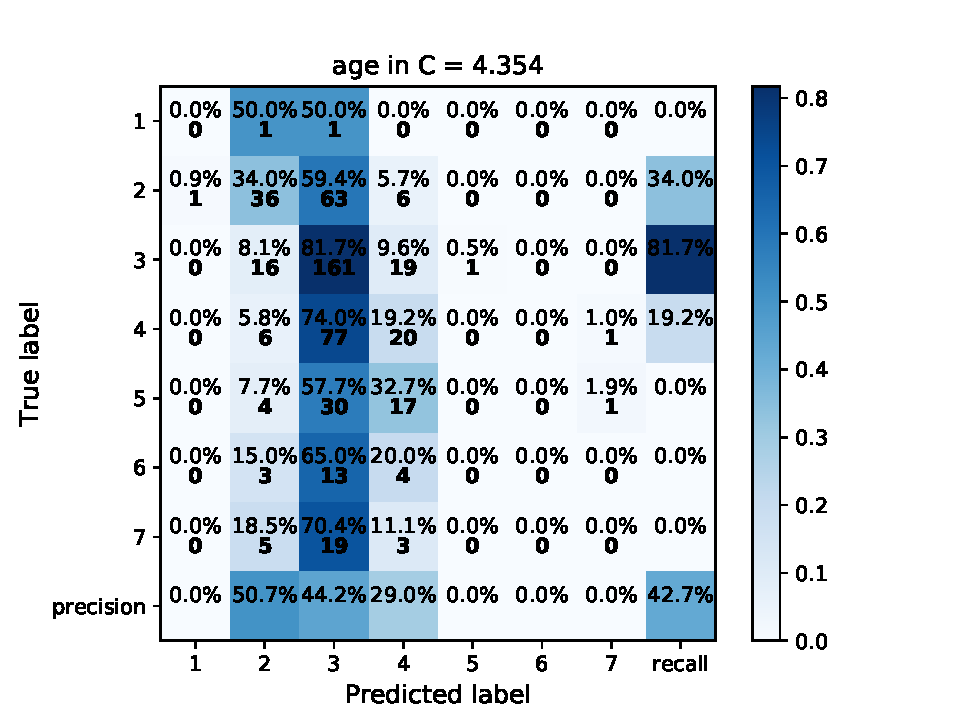
\includegraphics[scale=0.45]{fig/super_lr_age.pdf}
    \end{subfigure}%
    \begin{subfigure}
      \centering
      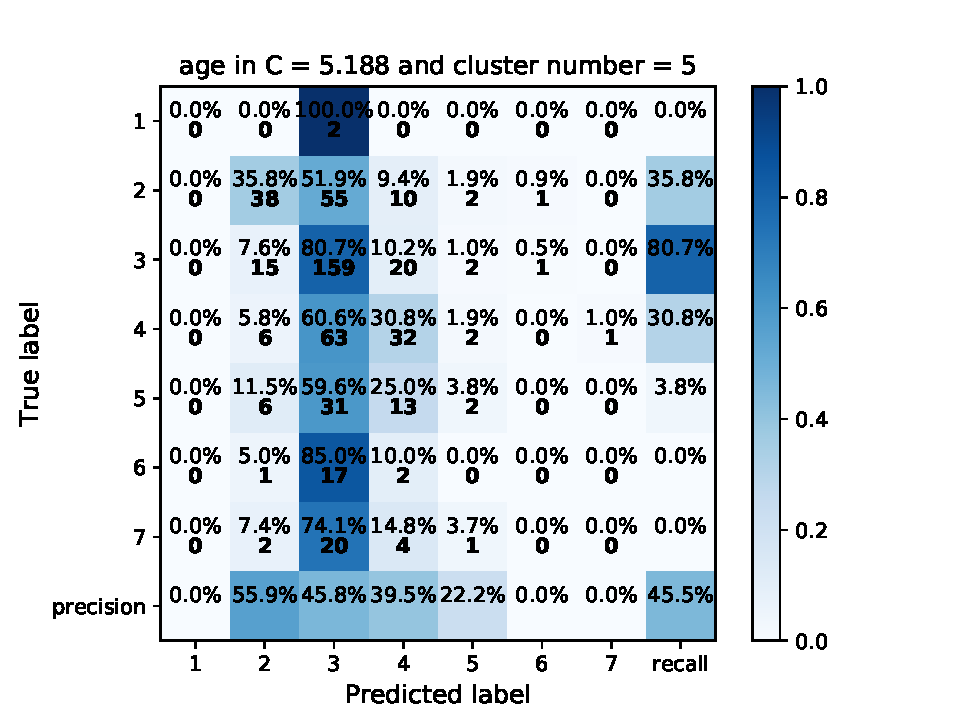
\includegraphics[scale=0.45]{fig/kms_lr_age.pdf}
    \end{subfigure}
\end{figure*}

\begin{figure*}[h]
    \centering
    \begin{subfigure}
      \centering
      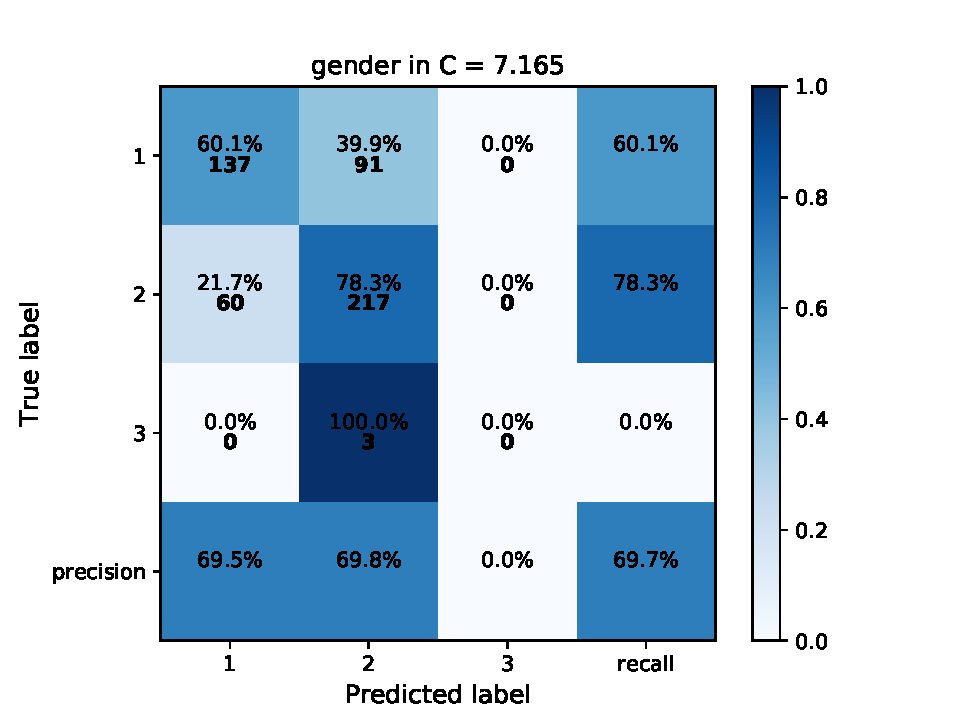
\includegraphics[scale=0.45]{fig/super_lr_gender.pdf}
    \end{subfigure}%
    \begin{subfigure}
      \centering
      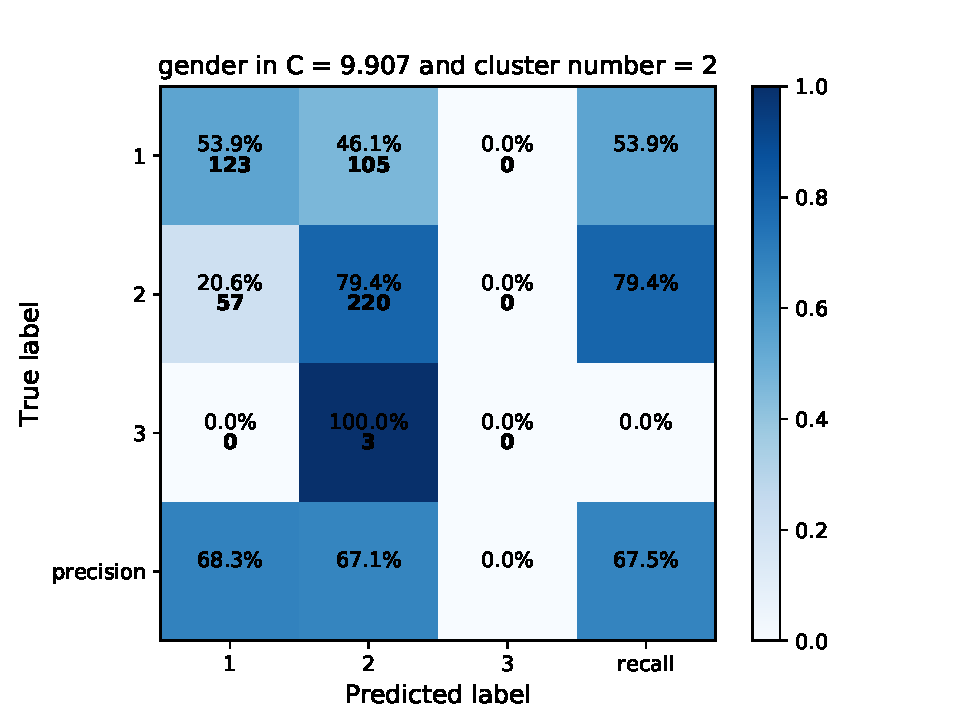
\includegraphics[scale=0.45]{fig/kms_lr_gender.pdf}
    \end{subfigure}
\end{figure*}

\begin{figure}[h]
    \centering
    \begin{subfigure}
      \centering
      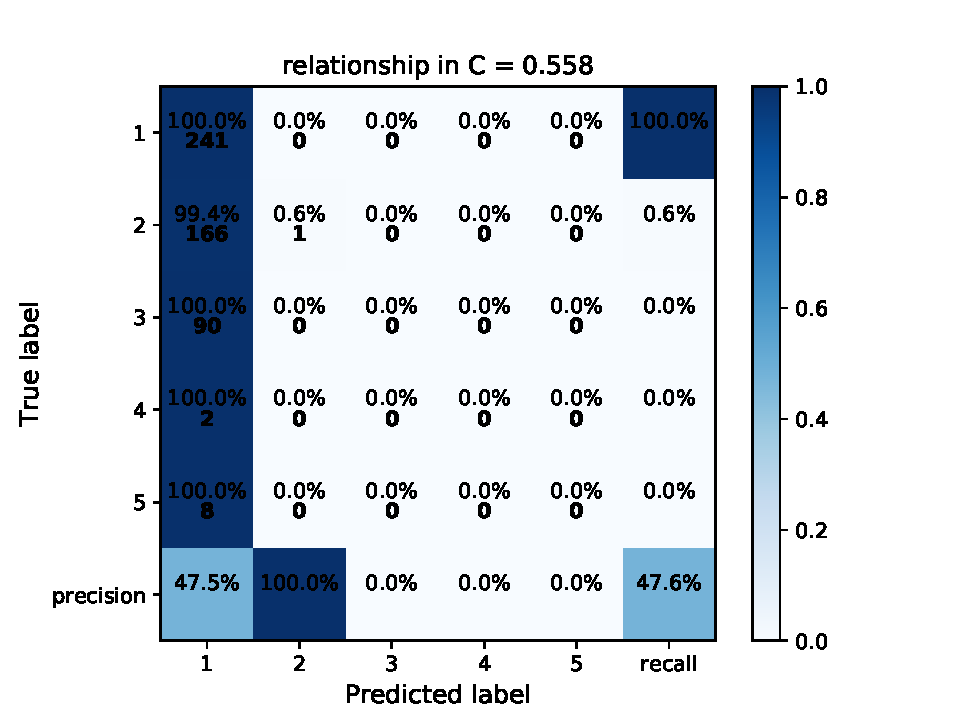
\includegraphics[scale=0.45]{fig/super_lr_relationship.pdf}
    \end{subfigure}%
    \begin{subfigure}
      \centering
      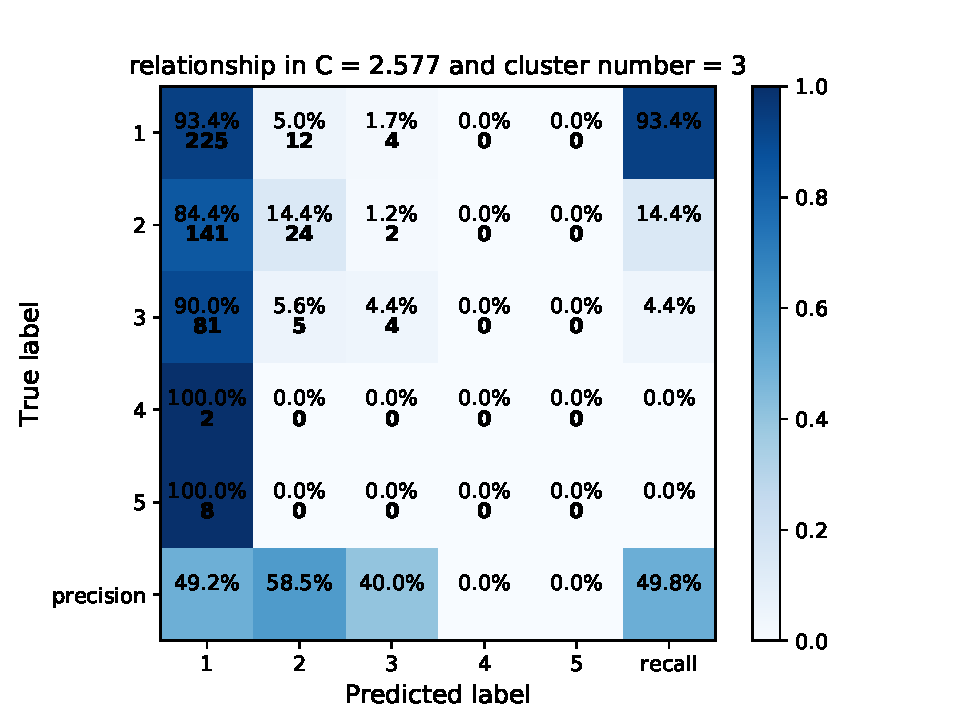
\includegraphics[scale=0.45]{fig/kms_lr_relationship.pdf}
    \end{subfigure}
    \caption{左側為 Logistic regression 預測個人資訊之混淆矩陣、右側為分群後以 Logistic regression 預測個人資訊之混淆矩陣}
    \label{fig:lr_con}
\end{figure}

\begin{figure*}[h]
    \centering
    \begin{subfigure}
      \centering
      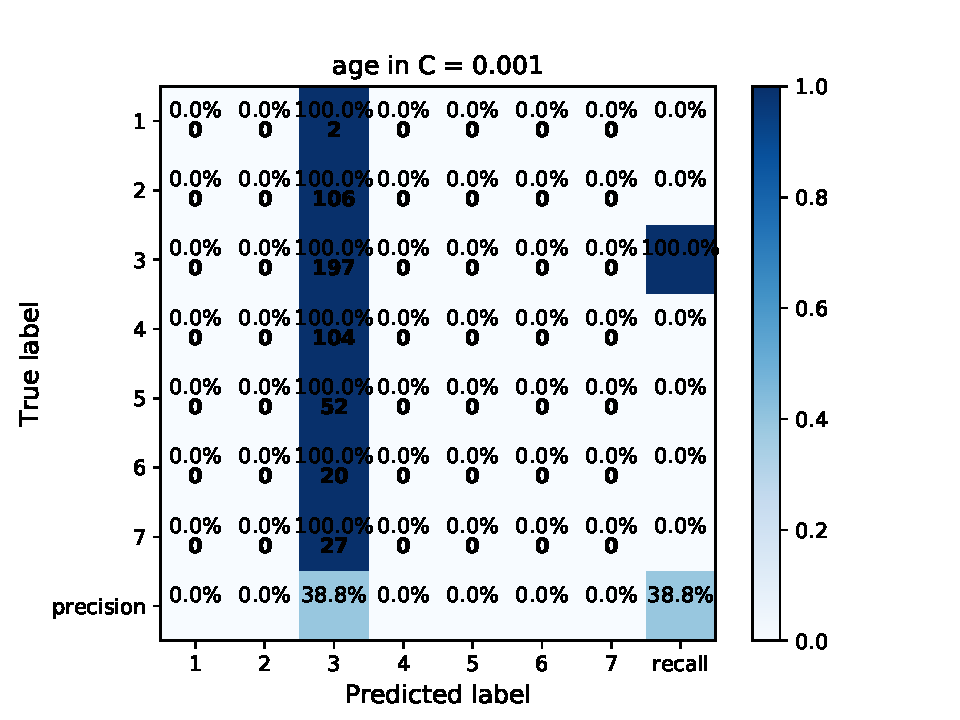
\includegraphics[scale=0.45]{fig/super_svm_age.pdf}
    \end{subfigure}%
    \begin{subfigure}
      \centering
      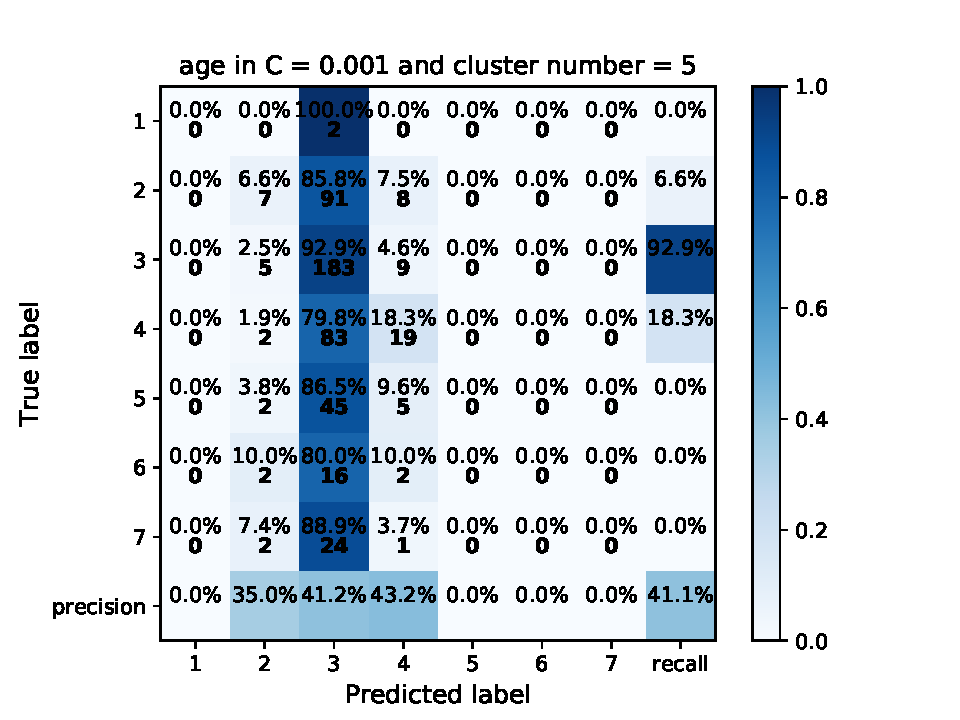
\includegraphics[scale=0.45]{fig/kms_svm_age.pdf}
    \end{subfigure}
\end{figure*}

\begin{figure*}[h]
    \centering
    \begin{subfigure}
      \centering
      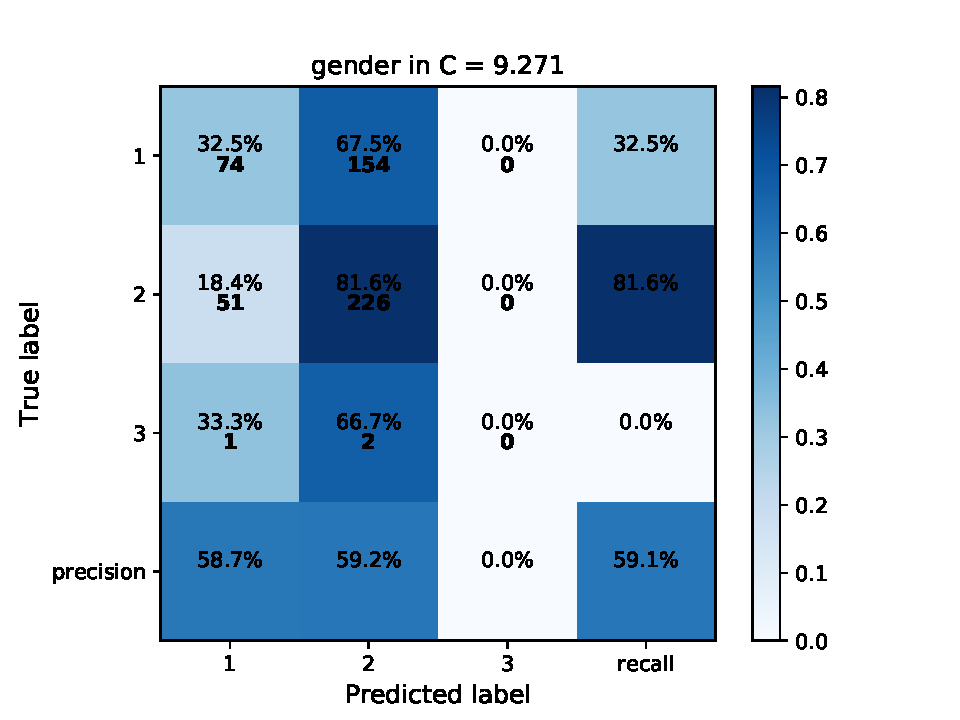
\includegraphics[scale=0.45]{fig/super_svm_gender.pdf}
    \end{subfigure}%
    \begin{subfigure}
      \centering
      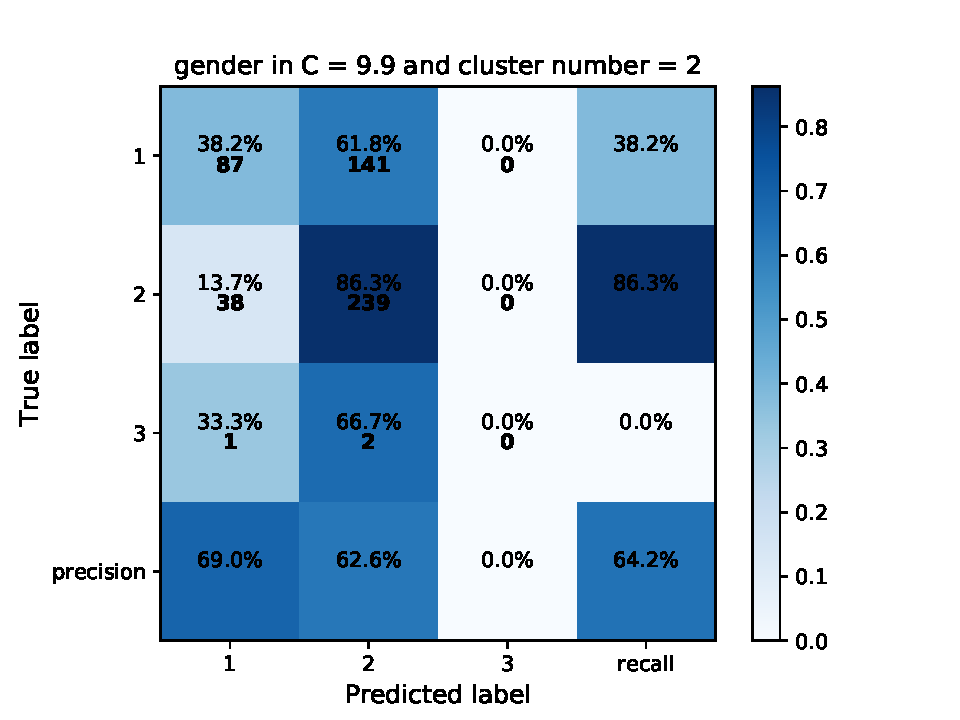
\includegraphics[scale=0.45]{fig/kms_svm_gender.pdf}
    \end{subfigure}
\end{figure*}

\begin{figure}[h]
    \centering
    \begin{subfigure}
      \centering
      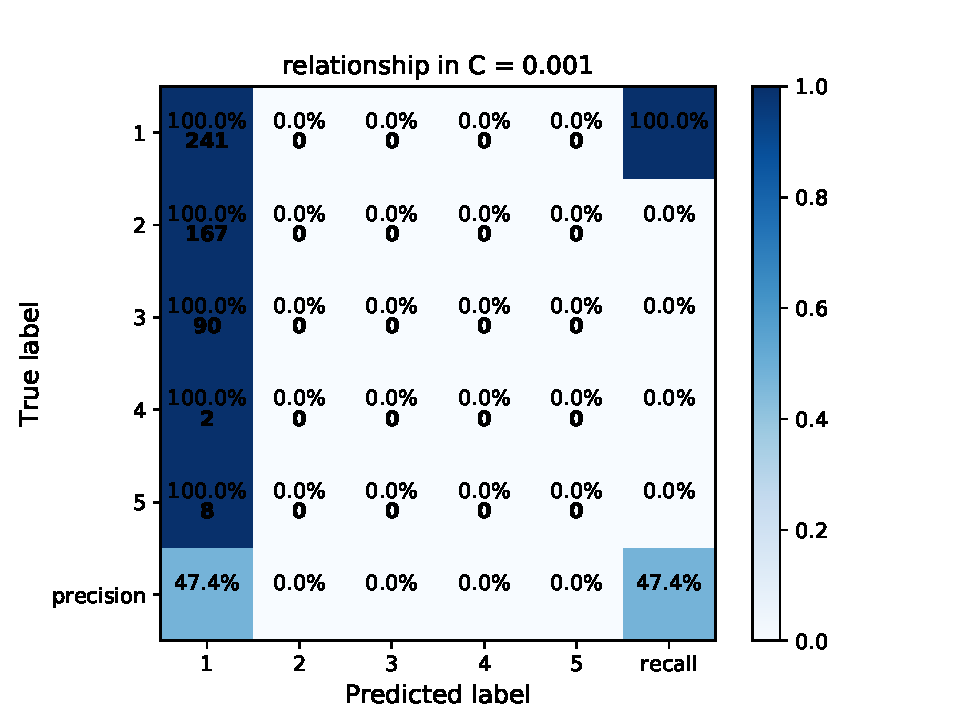
\includegraphics[scale=0.45]{fig/super_svm_relationship.pdf}
    \end{subfigure}%
    \begin{subfigure}
      \centering
      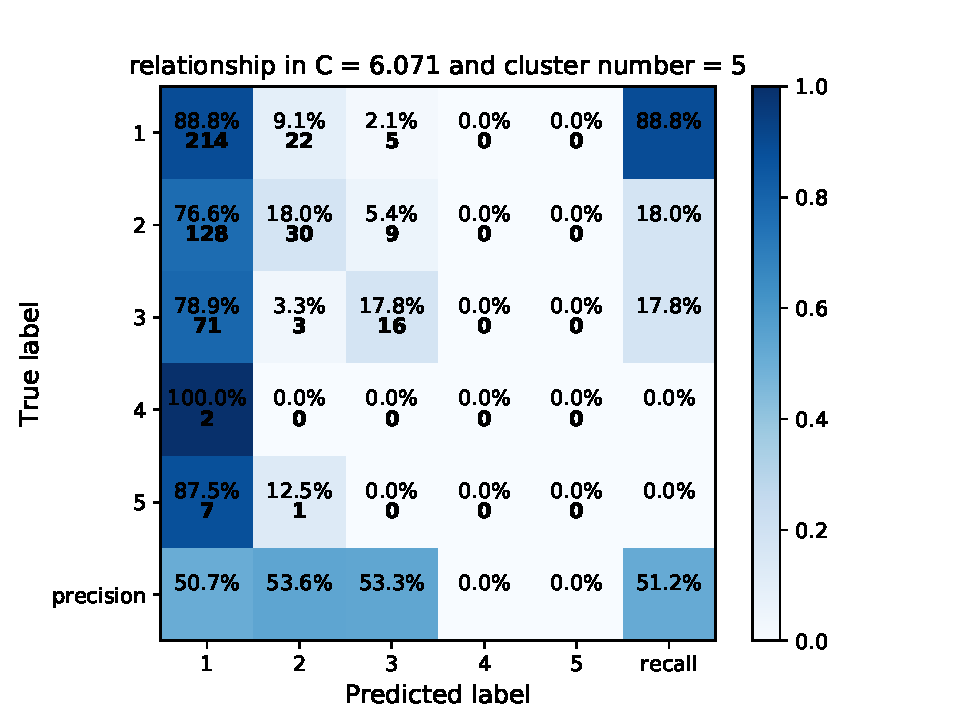
\includegraphics[scale=0.45]{fig/kms_svm_relationship.pdf}
    \end{subfigure}
    \caption{左側為 SVM 預測個人資訊之混淆矩陣、右側為分群後以 SVM 預測個人資訊之混淆矩陣}
    \label{fig:svm_con}
\end{figure}

}
\clearpage
\section{預測大六性格特質分數之結果比較}
{
本節將介紹以 $4$ 種方法:SVM、Lasso regression、Ridge regression 以及 Elastic net regression 之參數設定,並在最後以均方根誤差(root-mean-square error)比較 “基於監督式學習” 與 “結合分群之監督式學習” 兩者大六性格特質分數之預測結果。\par

基於監督式學習之預測方法中,使用 SVM 預測大六性格特質分數時能夠透過調整其中 regularization term 之權重($C$)來得到較低的 $RMSE$ 分數,其中盡責性(Conscientiousness)預測較準確($RMSE_{Con}=5.232$,$C=4.378$),而真誠性(Honesty-Humility)預測較差($RMSE_{HH}=5.789$,C=10)。而使用 Lasso regression、Ridge regression、Elastic net regression 預測大六性格特質分數時,同樣能透過調整 regularization term 之權重($Alpha$)來得到較佳的預測結果。Lasso regression 中預測盡責性(Conscientiousness)預測較準確($RMSE_{Con}=5.406$,$Alpha=0.001$),而外向性(Extraversion)預測較差($RMSE_{Ext}=5.881$,\\
$Alpha=0.001$)。Ridge regression 中預測盡責性(Conscientiousness)預測較準確($RMSE_{Con}=5.43$,$Alpha=0.001$),而情緒不穩定性(Neuroticism)預測較差($RMSE_{Neu}=5.981$,$Alpha=0.001$)。Elastic net regression 中預測盡責性(Conscientiousness)預測較準確($RMSE_{Con}=5.366$,$Alpha=0.001$),而真誠性(Honesty-Humility)預測較差($RMSE_{HH}=5.813$,$Alpha=0.001$)。詳細預測結果如表~\ref{tab:super_pr}。\par

\begin{table}[h]  
    \Large  
    \centering
    \fontsize{12}{20}\selectfont 
    \caption{基於監督式學習預測大六性格特質分數之結果}  
    \label{tab:super_pr}
    \begin{center}  
    \begin{tabular}{|l|l|l|l|l|}  
    \hline  
    Big-six personality& SVM & Lasso & Ridge & Elastic net \cr \hline  
    真誠性 & {\bf 5.789} & 5.832 & 5.845 & 5.813 \cr \hline  
    情緒不穩定性 & 5.78 & 5.87 & 5.981 & {\bf 5.769} \cr \hline 
    外向性 & 5.746 & 5.881 & 5.891 & {\bf 5.743} \cr \hline 
    親和性 & 5.643 & 5.71 & 5.795 & {\bf 5.622} \cr \hline 
    盡責性 & {\bf 5.232} & 5.406 & 5.43 & 5.366 \cr \hline 
    經驗開放性 & {\bf 5.38} & 5.607 & 5.646 & 5.44 \cr  
    \hline  
    \end{tabular}  
    \end{center}  
\end{table}  
\clearpage

結合分群之監督式學習的預測方法中,將使用者利用 k-means 將使用者分成 2 到 6 群後進行 SVM、Lasso regression、Ridge regression、Elastic net regression 進行大六性格特質分數之預測。使用 SVM 進行預測時,預測盡責性(Conscientiousness)預測較準確($RMSE_{Con}=5.048$,$C=9.353$,分群數$=4$),而情緒不穩定性(Neuroticism)預測較差($RMSE_{Neu}=5.623$,$C=9.53$,分群數$=4$)。使用 Lasso regression 進行預測時,預測盡責性(Conscientiousness)預測較準確($RMSE_{Con}=5.022$,$Alpha=0.245$,分群數$=4$),而情緒不穩定性(Neuroticism)預測較差($RMSE_{Neu}=5.469$,$Alpha=0.049$,分群數$=5$)。使用 Ridge regression 進行預測時,預測預測盡責性(Conscientiousness)預測較準確($RMSE_{Con}=5.027$,$Alpha=9.255$,分群數$=4$),而真誠性(Honesty-Humility)預測較差($RMSE_{HH}=5.43$,$Alpha=8.864$,分群數$=2$)。使用 Elastic net regression 進行預測時,預測盡責性(Conscientiousness)預測較準確($RMSE_{Con}=5.022$,$Alpha=0.398$,分群數$=4$),而外向性(Extraversion)預測較差($RMSE_{Ext}=5.422$,$Alpha=0.034$,分群數$=5$)。詳細預測結果如表~\ref{tab:kms_pr}。\par

\begin{table}[h]  
    \Large  
    \centering
    \fontsize{12}{20}\selectfont 
    \caption{結合分群之監督式學習預測大六性格特質分數結果}  
    \label{tab:kms_pr}
    \begin{center}  
    \begin{tabular}{|l|c|c|c|c|}  
    \hline  
    Big-six personality & SVM & Lasso & Ridge & Elastic net \cr \hline  
    真誠性 & 5.432 & {\bf 5.411} & 5.43 & 5.417 \cr \hline  
    情緒不穩定性 & 5.623 & 5.469 & 5.404 & {\bf 5.383} \cr \hline 
    外向性 & 5.402 & 5.435 & {\bf 5.38} & 5.422 \cr \hline 
    親和性 & 5.328 & 5.322 & 5.325 & {\bf 5.317} \cr \hline 
    盡責性 & 5.048 & {\bf 5.022} & 5.027 & {\bf 5.022} \cr \hline 
    經驗開放性 & 5.165 & 5.131 & {\bf 5.052} & 5.095 \cr  
    \hline  
    \end{tabular}  
    \end{center}  
\end{table} 
\clearpage

再透過比較 “將使用者分群後總是預測平均值(baseline)”、“基於監督式學習” 與 “結合分群之監督式學習” 大六性格特質分數之最佳預測結果(表~\ref{tab:total_pr}),可以了解結合分群之監督式學習之預測準確度在六種性格上皆高過基於監督式學習。

\begin{table}[h]  
    \Large  
    \centering
    \fontsize{12}{20}\selectfont 
    \caption{基於監督式學習與結合分群監督式學習之預測 $RMSE$ 分數比較表}  
    \label{tab:total_pr}
    \begin{center}  
    \begin{tabular}{|l|c|c|c|}  
    \hline  
    Big-six personality& Baseline & 基於監督式學習 & 結合分群監督式學習 \cr \hline  
    真誠性 & 5.806 & 5.789 & {\bf 5.411} \cr \hline  
    情緒不穩定性 & 5.718 & 5.769 & {\bf 5.383} \cr \hline 
    外向性 & 5.721 & 5.743 & {\bf 5.38} \cr \hline 
    親和性 & 5.604 & 5.622 & {\bf 5.317} \cr \hline 
    盡責性 & 5.224 & 5.232 & {\bf 5.022} \cr \hline 
    經驗開放性 & 5.281 & 5.38 & {\bf 5.052} \cr  
    \hline  
    \end{tabular}  
    \end{center}  
\end{table} 
}

\section{實驗結果分析}
\subsection{預測個人資訊結果分析}
{
k-NN 對於年齡方面的預測(圖~\ref{fig:knn_con} 中 age 部分),分群結果對於 $26\sim30$ 歲(Label:3)的使用者族群能夠更加準確被分類出來,但是對於 $21\sim25$ 歲(Label:2)的族群預測準確度明顯下降。性別方面相較年齡之預測效果更加成功,分群後預測準確度是 3 種個人資訊中效果提升最多的項目。而感情狀態中分群對於準確度幫助較少。\par

Random forests 對於年齡方面預測(圖~\ref{fig:rf_con} 中 age 部分)是 4 種分類器中效果最好的,但是分群後的準確度反而下降許多,但是對於 $21\sim25$ 歲(Label:2)的族群更能夠分類正確。性別方面(圖~\ref{fig:rf_con} 中 gender 部分),分群後對於女性(Label:2)分類效果較差,因此分群後反而整體準確度下降。而感情狀態(圖~\ref{fig:rf_con} 中 relationship 部分)中分群對於已婚(Label:3)的使用者能夠更加正確分類出來,因此整體預測效果上升許多。\par

Logistic regression 對於年齡方面的預測(圖~\ref{fig:lr_con} 中 age 部分)較於偏向分類為 $26\sim30$ 歲(Label:3),但是其中對於 $21\sim25$ 歲(Label:2)的族群反而是 4 種分類器中準確度最高的。性別方面(圖~\ref{fig:lr_con} 中 gender 部分)與 Random forests 類似,也是屬於分群後準確度降低的類型。而感情狀態方面(圖~\ref{fig:lr_con} 中 relationship 部分),總是預測使用者為單身(Label:1),而分群後由於訓練集中已婚(Label:3)的使用者所佔比例提升,因此對於已婚的使用者較能夠分類出來,所以整體準確度上升。\par

SVM 與 Logistic regression 預測結果有點類似,個人資訊中各方面都偏向預測樣本數最多的種類,而分群後較能夠預測出部分樣本數較少的使用者類別。由於偏向猜測樣本數最多的種類,因此與 baseline 預測分數較為類似。其中性別方面(圖~\ref{fig:svm_con} 中 gender 部分),分類器比較有學到正確的分類方式,因此預測結果比 baseline 高出許多。\par

綜合以上結果,分群對於感情狀態的分類效果比較幫助,4 種分類器經過分群準確度都有上升。而性別方面,預測準確度最高的為直接以 Random forests 與 Logistic regression 進行預測,而分群後之預測準確度反而下降,與原本預期中的結果不太相同。
}

\subsection{預測大六性格特質分數結果分析}
{
大六性格特質分數之預測中,SVM、Lasso、Ridge、Elastic net regression 之預測表現皆為結合分群的預測結果較好,其中 Lasso、Ridge、Elastic net regression 在分群之前對於 regularization term 都給予很小的權重,幾乎傾向做 regularization,但是在分群後則都對 regularization term 給予了不同的權重,表示分群對於使用線性回歸之預測有很大的幫助,而在最後的結果比較方面,也能夠明顯看出結合分群之效能有明顯提升。\par

其中比較特別的部分為 SVM 在未結合分群的狀態下,預測效果在真誠性、盡責性、經驗開放性是優於其他 3 種回歸方法的,而在結合分群之後 6 種性格特質分數中並沒有特別突出的表現,目前還找不到明確原因來解釋此現象。
}